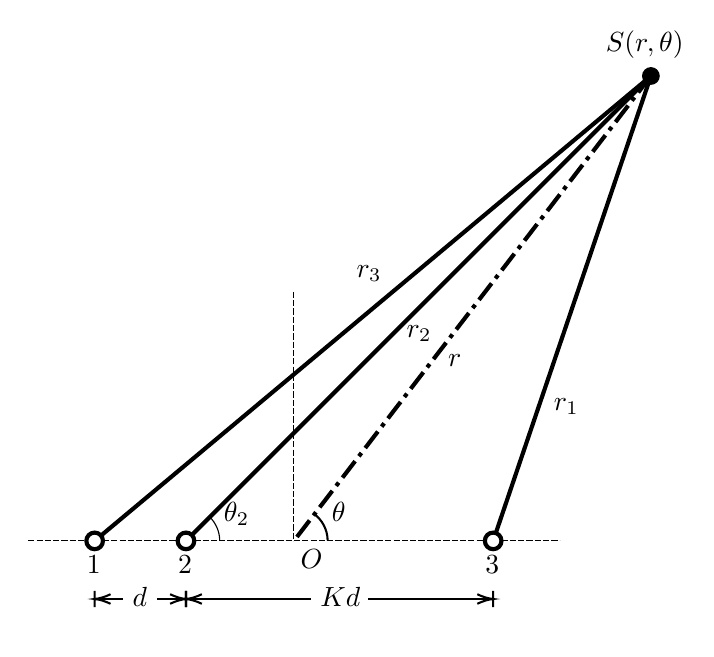
\begin{tikzpicture}[every picture/.style={line width=0.75pt}, x=0.75pt,y=0.75pt,yscale=-1,xscale=1]
    %uncomment if require: \path (0,318); %set diagram left start at 0, and has height of 318

    %Straight Lines [id:da042324791837329956]
    \draw [line width=1.5]    (244,268) -- (468,44) ;
    %Straight Lines [id:da7482650625206233]
    \draw [line width=1.5]    (468,44) -- (392,268) ;
    %Straight Lines [id:da8759803470570984]
    \draw  [dash pattern={on 2.25pt off 0.75pt}]  (168,268) -- (424,268) ;
    %Straight Lines [id:da3612564917664043]
    \draw  [dash pattern={on 2.25pt off 0.75pt}]  (296,148) -- (296,268) ;

    %Shape: Circle [id:dp701214228276472]
    \draw  [fill={rgb, 255:red, 0; green, 0; blue, 0 }  ,fill opacity=1 ] (464,44) .. controls (464,41.79) and (465.79,40) .. (468,40) .. controls (470.21,40) and (472,41.79) .. (472,44) .. controls (472,46.21) and (470.21,48) .. (468,48) .. controls (465.79,48) and (464,46.21) .. (464,44) -- cycle ;
    %Straight Lines [id:da46776944434905854]
    \draw [line width=1.5]    (468,44) -- (200,268) ;
    %Shape: Circle [id:dp41637404945939793]
    \draw  [fill={rgb, 255:red, 255; green, 255; blue, 255 }  ,fill opacity=1 ][line width=1.5]  (388,268) .. controls (388,265.79) and (389.79,264) .. (392,264) .. controls (394.21,264) and (396,265.79) .. (396,268) .. controls (396,270.21) and (394.21,272) .. (392,272) .. controls (389.79,272) and (388,270.21) .. (388,268) -- cycle ;
    %Shape: Circle [id:dp3472405999942534]
    \draw  [fill={rgb, 255:red, 255; green, 255; blue, 255 }  ,fill opacity=1 ][line width=1.5]  (196,268) .. controls (196,265.79) and (197.79,264) .. (200,264) .. controls (202.21,264) and (204,265.79) .. (204,268) .. controls (204,270.21) and (202.21,272) .. (200,272) .. controls (197.79,272) and (196,270.21) .. (196,268) -- cycle ;
    %Straight Lines [id:da8463556712184459]
    \draw [line width=1.5]  [dash pattern={on 7.5pt off 2.25pt on 1.5pt off 2.25pt}]  (468,44) -- (296,268) ;
    %Shape: Arc [id:dp41353820710334777]
    \draw  [draw opacity=0][line width=0.75]  (305.66,254.93) .. controls (309.58,257.84) and (312.15,262.46) .. (312.25,267.68) -- (296,268) -- cycle ; \draw  [line width=0.75]  (305.66,254.93) .. controls (309.58,257.84) and (312.15,262.46) .. (312.25,267.68) ;
    %Shape: Arc [id:dp19292277101405086]
    \draw  [draw opacity=0] (255.44,256.46) .. controls (258.34,259.33) and (260.16,263.29) .. (260.25,267.68) -- (244,268) -- cycle ; \draw   (255.44,256.46) .. controls (258.34,259.33) and (260.16,263.29) .. (260.25,267.68) ;
    %Straight Lines [id:da8674403841051044]
    \draw    (200,296) -- (244,296) ;
    \draw [shift={(244,296)}, rotate = 180] [color={rgb, 255:red, 0; green, 0; blue, 0 }  ][line width=0.75]    (0,3.91) -- (0,-3.91)(7.65,-2.3) .. controls (4.86,-0.97) and (2.31,-0.21) .. (0,0) .. controls (2.31,0.21) and (4.86,0.98) .. (7.65,2.3)   ;
    \draw [shift={(200,296)}, rotate = 0] [color={rgb, 255:red, 0; green, 0; blue, 0 }  ][line width=0.75]    (0,3.91) -- (0,-3.91)(7.65,-2.3) .. controls (4.86,-0.97) and (2.31,-0.21) .. (0,0) .. controls (2.31,0.21) and (4.86,0.98) .. (7.65,2.3)   ;
    %Shape: Circle [id:dp45604077591200665]
    \draw  [fill={rgb, 255:red, 255; green, 255; blue, 255 }  ,fill opacity=1 ][line width=1.5]  (240,268) .. controls (240,265.79) and (241.79,264) .. (244,264) .. controls (246.21,264) and (248,265.79) .. (248,268) .. controls (248,270.21) and (246.21,272) .. (244,272) .. controls (241.79,272) and (240,270.21) .. (240,268) -- cycle ;
    %Straight Lines [id:da3454693803086273]
    \draw    (244,296) -- (392,296) ;
    \draw [shift={(392,296)}, rotate = 180] [color={rgb, 255:red, 0; green, 0; blue, 0 }  ][line width=0.75]    (0,3.91) -- (0,-3.91)(7.65,-2.3) .. controls (4.86,-0.97) and (2.31,-0.21) .. (0,0) .. controls (2.31,0.21) and (4.86,0.98) .. (7.65,2.3)   ;
    \draw [shift={(244,296)}, rotate = 0] [color={rgb, 255:red, 0; green, 0; blue, 0 }  ][line width=0.75]    (0,3.91) -- (0,-3.91)(7.65,-2.3) .. controls (4.86,-0.97) and (2.31,-0.21) .. (0,0) .. controls (2.31,0.21) and (4.86,0.98) .. (7.65,2.3)   ;

    % Text Node
    \draw (387,274) node [anchor=north west][inner sep=0.75pt]   [align=left] {3};
    % Text Node
    \draw (195,274) node [anchor=north west][inner sep=0.75pt]   [align=left] {1};
    % Text Node
    \draw (420,198) node [anchor=north west][inner sep=0.75pt]   [align=left] {$\displaystyle r_{1}$};
    % Text Node
    \draw (349,163) node [anchor=north west][inner sep=0.75pt]   [align=left] {$\displaystyle r_{2}$};
    % Text Node
    \draw (325,134) node [anchor=north west][inner sep=0.75pt]   [align=left] {$\displaystyle r_{3}$};
    % Text Node
    \draw (369,177) node [anchor=north west][inner sep=0.75pt]   [align=left] {$\displaystyle r$};
    % Text Node
    \draw (313,248) node [anchor=north west][inner sep=0.75pt]   [align=left] {$\displaystyle \theta $};
    % Text Node
    \draw (261,248) node [anchor=north west][inner sep=0.75pt]   [align=left] {$\displaystyle \theta _{2}$};
    % Text Node
    \draw (445,21) node [anchor=north west][inner sep=0.75pt]   [align=left] {$\displaystyle S( r,\theta )$};
    % Text Node
    \draw  [color={rgb, 255:red, 255; green, 255; blue, 255 }  ,draw opacity=1 ][fill={rgb, 255:red, 255; green, 255; blue, 255 }  ,fill opacity=1 ]  (214,285) -- (230,285) -- (230,310) -- (214,310) -- cycle  ;
    \draw (217,289) node [anchor=north west][inner sep=0.75pt]   [align=left] {$\displaystyle d$};
    % Text Node
    \draw  [color={rgb, 255:red, 255; green, 255; blue, 255 }  ,draw opacity=1 ][fill={rgb, 255:red, 255; green, 255; blue, 255 }  ,fill opacity=1 ]  (304.5,285) -- (331.5,285) -- (331.5,310) -- (304.5,310) -- cycle  ;
    \draw (307.5,289) node [anchor=north west][inner sep=0.75pt]   [align=left] {$\displaystyle Kd$};
    % Text Node
    \draw (298,271) node [anchor=north west][inner sep=0.75pt]   [align=left] {$\displaystyle O$};
    % Text Node
    \draw (239,274) node [anchor=north west][inner sep=0.75pt]   [align=left] {2};


\end{tikzpicture}